\documentclass[sigconf,9pt]{acmart}
\usepackage[utf8]{inputenc}
\usepackage{amsmath}
\usepackage{amsfonts}
%\usepackage{amssymb}
\usepackage{amsthm}
\usepackage{graphicx}
%\usepackage{xcolor}
%\usepackage{soul}
%\usepackage{hyperref}
\usepackage{algorithm}
\usepackage[noend]{algpseudocode}
%\usepackage{dsfont}
%\usepackage[font=small, labelfont=bf]{caption}
%\usepackage[left=2cm,right=2cm,top=2cm,bottom=2cm]{geometry}
\usepackage{subcaption}
\usepackage{todonotes}
\usepackage{multirow}
\usepackage{enumitem}
\usepackage{tablefootnote}
\usepackage{placeins}
\newcommand\el[1]{\textcolor{orange}{{\bf Erick: }#1}}

\newcommand\ssbtokens[0]{\textit{SSB-Tokens} }
\newcommand\invpathcomment[0]{
\begin{flushleft}
{\color{commentgray}\textit{Msg} refers to enclosing SSB message. Properties (in italics) without an explicit access path refer to the operation properties stored in \textit{msg.content}. See implementation for other requirements not related to the paper arguments.} 
\label{req:comment}
\end{flushleft}}

\newcommand\idemcomment[0]{
\begin{flushleft}
{\color{commentgray} \textit{Idem} comment (see Req.~\ref{req:comment}).}
\end{flushleft}}

\newcommand{\mylabel}[2]{#2\def\@currentlabel{#2}\label{#1}}

\floatstyle{ruled}
\newfloat{invariants}{th}{inv}
\floatname{invariants}{Requirements}

\definecolor{commentgray}{gray}{0.28}

\hyphenation{block-chain}
\hyphenation{block-chains}
\hyphenation{Ethe-reum}


\renewcommand{\copyrightpermissionfootnoterule}{%
\hrule
 \vspace*{-1pt}
  \noindent%
\\
\hfill
  
\includegraphics[width=0.16\columnwidth]{creative-commons-by_sa_4_0}
 \hfill
  \begin{minipage}[b]{0.82\columnwidth}
    \footnotesize 

This work is licensed under a Creative Commons Attribution ShareAlike International 4.0 License.
  \end{minipage}%
  \vspace*{2pt}%
\hrule
  \vspace*{2pt}
}

\acmYear{2022}
\copyrightyear{2022}
\setcopyright{rightsretained} 
\acmConference[DICG '22]{3rd International Workshop on Distributed Infrastructure for the Common Good}{November 7, 2022}{Quebec, QC, Canada}
\acmBooktitle{3rd International Workshop on Distributed Infrastructure for the Common Good (DICG '22), November 7, 2022, Quebec, QC, Canada}
\acmDOI{10.1145/3565383.3566113}
\acmISBN{978-1-4503-9928-9/22/11}

\begin{CCSXML}
<ccs2012>
   <concept>
       <concept_id>10010520.10010521.10010537.10010540</concept_id>
       <concept_desc>Computer systems organization~Peer-to-peer architectures</concept_desc>
       <concept_significance>500</concept_significance>
       </concept>
   <concept>
       <concept_id>10003120</concept_id>
       <concept_desc>Human-centered computing</concept_desc>
       <concept_significance>500</concept_significance>
       </concept>
   <concept>
       <concept_id>10010147.10010919.10010172</concept_id>
       <concept_desc>Computing methodologies~Distributed algorithms</concept_desc>
       <concept_significance>500</concept_significance>
       </concept>
   <concept>
       <concept_id>10010405.10003550.10003551</concept_id>
       <concept_desc>Applied computing~Digital cash</concept_desc>
       <concept_significance>500</concept_significance>
       </concept>
 </ccs2012>
\end{CCSXML}

\ccsdesc[500]{Computer systems organization~Peer-to-peer architectures}
\ccsdesc[500]{Human-centered computing}
\ccsdesc[500]{Computing methodologies~Distributed algorithms}
\ccsdesc[500]{Applied computing~Digital cash}

\keywords{economics, peer-to-peer, crypto-tokens, blockchain, local economics, producer credit}

\begin{document}


\title{Local Crypto-Tokens for Local Economics}

\author{Erick Lavoie}
\email{erick.lavoie@unibas.ch}
\affiliation{%
  \institution{University of Basel, Basel, Switzerland}
}

\author{Christian Tschudin}
\email{christian.tschudin@unibas.ch}
\affiliation{%
  \institution{University of Basel, Basel, Switzerland}
}


\begin{abstract}
Major blockchain projects, such as Bitcoin and Ethereum, enable secure global transfers of tokens between untrusted parties. The resulting global financial infrastructure however incurs latency and costs that are prohibitive for many economics applications that are local to a region or a community. Local economics relies on trust and reputation through repeated interactions within a community of participants that know each other, which has not previously been leveraged for the design of crypto-tokens. In this paper, we formulate the design of new \textit{local crypto-tokens} as a research problem: we present concrete application examples, we identify double-spending detection as a weaker and sufficient alternative to double-spending prevention in local applications, and we formulate desired properties of new local crypto-tokens designs. Based on our analysis, we envision local crypto-tokens to complement existing blockchain projects by facilitating intra-community economics at much lower latency and costs, while evolutions of current blockchain projects will provide global inter-community exchanges of high-value transactions.
\end{abstract}

\maketitle

\section{Introduction}

Major blockchain projects, such as Bitcoin~\cite{nakamoto2008bitcoin} and Ethereum~\cite{buterin2014next}, implement \textit{global financial infrastructure}, respectively as a replicated ledger or as a replicated state-machine. In both cases, creating new tokens, by forking an existing project or implementing them as smart-contracts, requires specialized technical skills. Moreover, maintaining the integrity of transactions demands Internet connectivity, and requires significant energy\footnote{Estimated at 2.2MWh per transaction in April 2022~\cite{bitcoin-transaction-energy}, approximately equivalent to 4 months of total electricity consumption of a Swiss person on average in 2015~\cite{average-energy-consumption-per-capita-ch}.}~\cite{vranken2017sustainability,sedlmeir2020energy} or capital stake\footnote{In June 2022, total staked Ethereum tokens for the purpose of block mining are worth in the order of 15 Billions USD~\cite{proof-of-stake}.}~\cite{sedlmeir2020energy}. The resulting costs become prohibitive for many applications that are inherently \textit{local} to a region or community.

For those applications, we propose instead to \textit{localize} the operations of crypto-token infrastructure in multiple complementary ways: (1) The creation of tokens is done by specific identities and authenticated, preventing any other identity to forge tokens for a different identity, foregoing the need for a global mining process; (2) The value of each specific token derives from the trust that their creator will fulfill the obligations they have linked to the tokens, instead of the demand for an abstract supply-limited token; (3) Transactions are public to a \textit{local} community, \textit{e.g.}, linked to a geographical region or bound by common interest, and recorded on local logs, instead of globally shared on a single global ledger; (4) Double-spending is \textit{detected} rather than prevented, through immutable proofs linked to a specific identity, and the cost of fraud is ultimately the exclusion of that identity from future participation in the community (worth more than the value of most transactions). Compared to Bitcoin or Ethereum-based alternatives, localizing the operations has the potential to simplify the implementation of crypto-tokens by replacing much of the technical or capital costs of maintaining transaction integrity with social trust and reputation, yet still enables a large variety of local applications to be supported.

In this paper, \textit{we identify an unexplored part of the space for crypto-token designs in support of local economics, for which existing crypto-currencies are ill-suited, and formulate it as a research problem}. Our goal is to motivate new designs and implementations that can leverage the trust and reputation built (or lost) within a community. We envision \textit{local crypto-tokens} to solve the need for \textit{intra-community} economics at significantly lower latency and costs than existing solutions while evolutions of existing blockchain projects will support global high-valued \textit{inter-communities} exchanges.

In the rest of this paper, we first start with a motivating example (Section~\ref{section:motivation}) to show some limitations of existing blockchain projects. We then present the \textit{detection} of double-spending as a weaker but sufficient alternative to double-spending prevention in a local context and show several examples (Section~\ref{section:double-spending}). We further summarize key dimensions for the design of crypto-tokens for local economics (Section~\ref{section:problem}). We then present additional applications that would benefit from solving this problem (Section~\ref{section:applications}), we relate this problem to other works (Section~\ref{section:related-work}), and we briefly conclude with perspectives for future work (Section~\ref{section:conclusion}).


\section{Motivation: Fidelity Card in a Small Shop}
\label{section:motivation}

Consider a \textit{sandwich shop} that offers a fidelity card to its customers, with one stamp added on the card for each sandwich bought. After 10 stamps, customers can exchange the full card for a free sandwich. This is a common real-world business strategy that is most usually thought of as marketing but is also a form of currency design.

In effect, through this fidelity card program, the owner introduces a \textit{shop-specific currency}, that is only redeemable for sandwiches in his shop. Each token, in the form of an ink stamp made with a custom or hard-to-find rubber stamp,  is worth one-tenth of a sandwich and represents \textit{a promise} from the shop owner to offer sandwiches in the future in exchange for a sufficient number of tokens. A new token is created every time a stamp is put on a card. The total supply of tokens has no a priori bound and grows with the number of customers that choose to use the fidelity cards. In one particular example we found,\footnote{From private discussions with the \textit{Ty Chaud} shop owner in Grenoble (France): \newline \url{http://tychaud.fr}.} the shop owner allows customers to redeem sandwiches using ten stamps collected in potentially multiple cards, even if the cards were partially filled by different customers: this effectively allows his customers to gift their incomplete cards to others. Once a customer redeems a sandwich in exchange for cards worth 10 stamps, the owner destroys the card(s). The lifetime of a token therefore ends with the destruction of the cards, either with the fulfillment of the underlying promise for a sandwich, or by destruction of the cards by others than the shop owner. Transactions with fidelity cards are instantaneous and free, and the material to run the program costs tens of Euros.

\subsection{Comparison to Bitcoin and Ethereum}

Contrast the above to the operations of a Bitcoin or Ethereum infrastructure. In the case of Bitcoin, the tokens are created by \textit{miners} and there is an \textit{upper bound} on the total amount of coins in circulation. 
The value of Bitcoin is partially determined by its ability to store wealth and appreciate in value, based on growth in demand against a \textit{fixed number of tokens}. To use Bitcoins as tokens in a fidelity card, the shop owner would have to acquire them first in exchange for money. Acquiring tokens would take at least 10 minutes, and more likely at least 30 minutes to ensure enough blocks were confirmed. Transferring tokens to customers would require an Internet connection, transaction fees, and again 30 minutes of wait for confirmation. In the case of Ethereum, the shop owner could instead create one or multiple \textit{smart-contracts}, allowing the contracts to create as many shop-specific tokens as needed. However, transfers to customers would still require an Internet connection, transaction fees (in Ethereum tokens), and transfer confirmations would take at least a minute or so. % Moreover, the creation of \textit{correct} smart-contracts requires programming skills that are beyond those of most shop owners. The costs of transactions and hourly wages to hire a programmer to maintain the fidelity cards would most likely consume all of the economic benefits of the fidelity card program. % Tokens are not usually intentionally destroyed, but may be lost or burned by sending to an invalid receiver address.

In effect, the Bitcoin and Ethereum-based financial infrastructures are ill-suited because they actually solve a different and much harder problem than is required for implementing a fidelity card program: Bitcoin and Ethereum provide \textit{secure global transfers of tokens between untrusting parties}. In our shop example instead, the economic activity is \textit{local} and tied to a \textit{neighbourhood}, both limited in the geographical area it covers and the number of participants. There is no real need and little benefit to broadcasting fidelity card transactions to the entire world on a single ledger. The participants know each other, at least in their direct transactions with the sandwich shop. The value of tokens derives from \textit{trust} that the token emitter, \textit{e.g.}, the shop owner, will actually fulfill the associated promises in the future, \textit{e.g.}, offer free sandwiches. 

A fidelity card program, made with paper cards and rubber stamps, is usually reserved for items of small value because it is not that difficult for customers to buy or create a similar rubber stamp and ink, and therefore \textit{forge} new tokens without actually buying sandwiches. However, with public-key cryptography and recent peer-to-peer gossiping systems, it is actually possible to achieve similar ease in token creation, fast transfers, and no transaction fees as in a fidelity card program but with stronger security properties: we can \textit{bind the token creation to a specific author}, such as the fidelity points created by a shop owner; we can design other operations such that other participants \textit{cannot forge} new tokens but only refer to those created by the original author.  The increased level of security then enables additional applications for shop owners such as self-emitted electronic gift cards, or community crowdfunding (Section~\ref{section:community-crowdfunding}), using a single system. Moreover, public trading of local tokens would increase the visibility of the participating shops.\footnote{From private discussions with the \textit{Ty Chaud} shop owner, additional visibility is what made them most interested in \textit{local crypto-tokens}.}

However, binding the tokens to a specific author is not sufficient to obtain a secure token system, because there can still be possibilities of \textit{double-spending}, \textit{i.e.}, transferring the same tokens to multiple participants, which we discuss next. 



\section{Double-Spending}
\label{section:double-spending}

To see how double-spending may arise, let's first consider a hypothetical  fidelity card program built on a gossiping system that replicates \textit{append-only logs}, such as Secure-Scuttlebutt (SSB)~\cite{kermarrec2020gossiping}. Participants have identifiers, written as \textit{@id}, which corresponds to their public key and they authenticate their messages with their corresponding private key, by signing the messages. Each new message signed also includes a pointer to the last message signed by the same \textit{author} and a strictly increasing \textit{sequence number} representing the index of the new message in the log.  When two participants meet locally, or optionally connect over the Internet, they replicate each other's log as well as those of other mutually-known participants~\cite{kermarrec2020gossiping}.

Figure~\ref{figure:example} shows one sequence of events between a customer and a shop owner illustrating transactions related to a fidelity card program.  The yellow boxes represent events happening in the real world, while the blue boxes represent operations recorded on the logs, respectively of the shop owner (\textit{@shop}) and a regular customer (\textit{@customer}). In this example, the shop owner, in addition to giving a sandwich in exchange for $5$ Euros, also creates then gives  a "Shop Point" to the customer. Once the customer has received 10 "Shop Points", the customer transfers the points to the shop owner to obtain a free sandwich. The shop owner then burns the points, as the underlying promise of a free sandwich has been redeemed.

\begin{figure}[htbp]
\centering
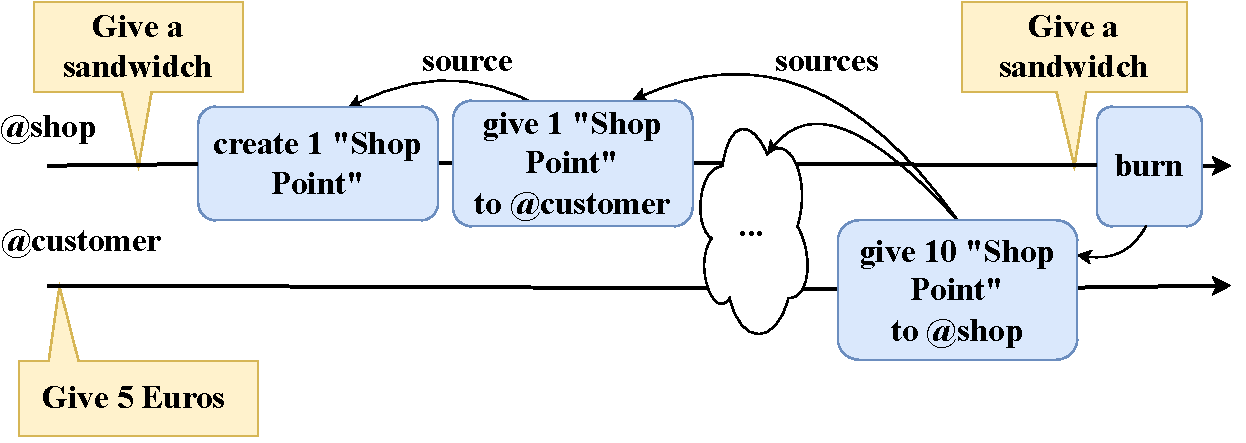
\includegraphics[width=0.48\textwidth]{./figures/example-drawio}
\caption{Example of crypto-token operations on append-only logs in blue and real-world events in yellow.}
\label{figure:example}
\end{figure}

Because participants are free to record any kind of operation in their logs, they may actually record operations in which they give the same tokens to multiple participants. Figure~\ref{figure:double-spend} illustrates one instance in which a customer, \textit{@eve}, gives the same tokens to two different participants, \textit{@alice} and \textit{@bob}, by using the same source in both operations. However, since both operations were immutably recorded in \textit{@eve}'s log, and the messages were both signed by her, there is actually an \textit{immutable proof of double-spending}. This proof can be shared to other participants by flagging all the operations that were involved in the fraudulent transactions. In this example, the first operation to \textit{@alice} would be valid because up-to-that sequence number in the log, there was no double-spending. However, the second operation to \textit{@bob} is  invalid because it spends tokens beyond what was available in the source. Because of the log structure, in which later messages point to the earlier messages (and have higher sequence numbers), there is a clear \textit{happened-before} relationship between the first and second transactions so only the second is invalid.

\begin{figure}[htbp]
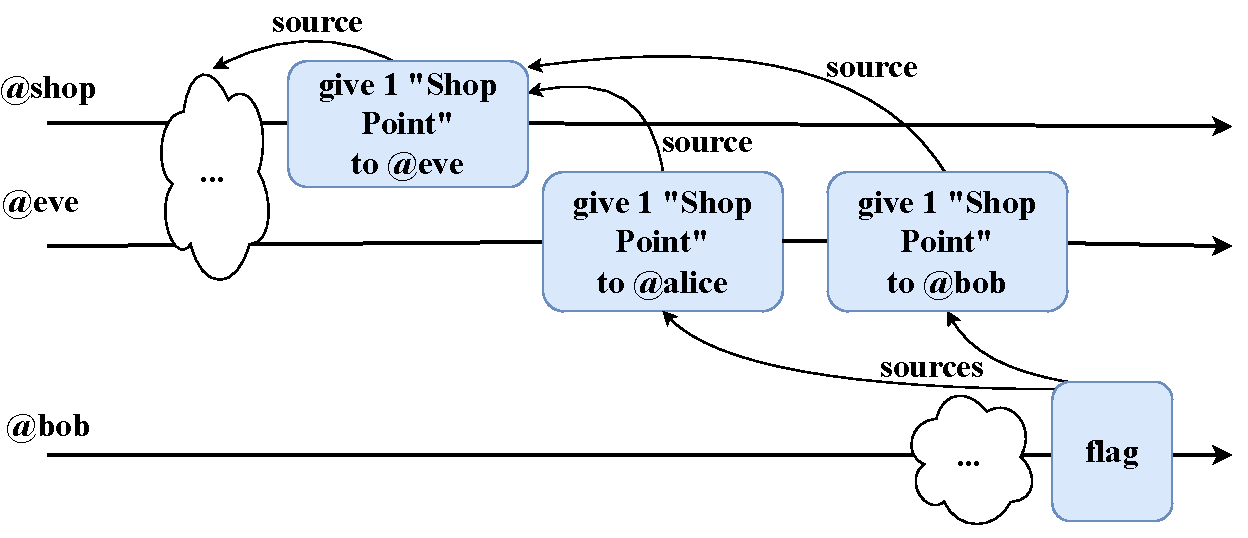
\includegraphics[width=0.48\textwidth]{figures/double-spend-drawio}
\caption{Double-Spend}
\label{figure:double-spend}
\end{figure}

A more subtle example of double-spending is illustrated in Figure~\ref{figure:fork-double-spend}, in which \textit{@eve} presents \textit{different logs} to two other participants and can therefore rewrite the operation at sequence number 100 to give tokens twice, both to \textit{@alice} and \textit{@bob}. This cannot be detected by other participants if they only have an interaction with \textit{@eve}. However, again because the messages are signed, eventually \textit{@alice} and \textit{@bob} would replicate their local copy of \textit{@eve}'s log, either directly or through other participants in the community. The inconsistency will eventually be found and it suffices to flag the identifiers of all messages creating new forks. In this case however, there is no clear \textit{happened-before} relationship between the two operations involved in double-spending, therefore both would be considered invalid.

\begin{figure}[htbp]
\centering
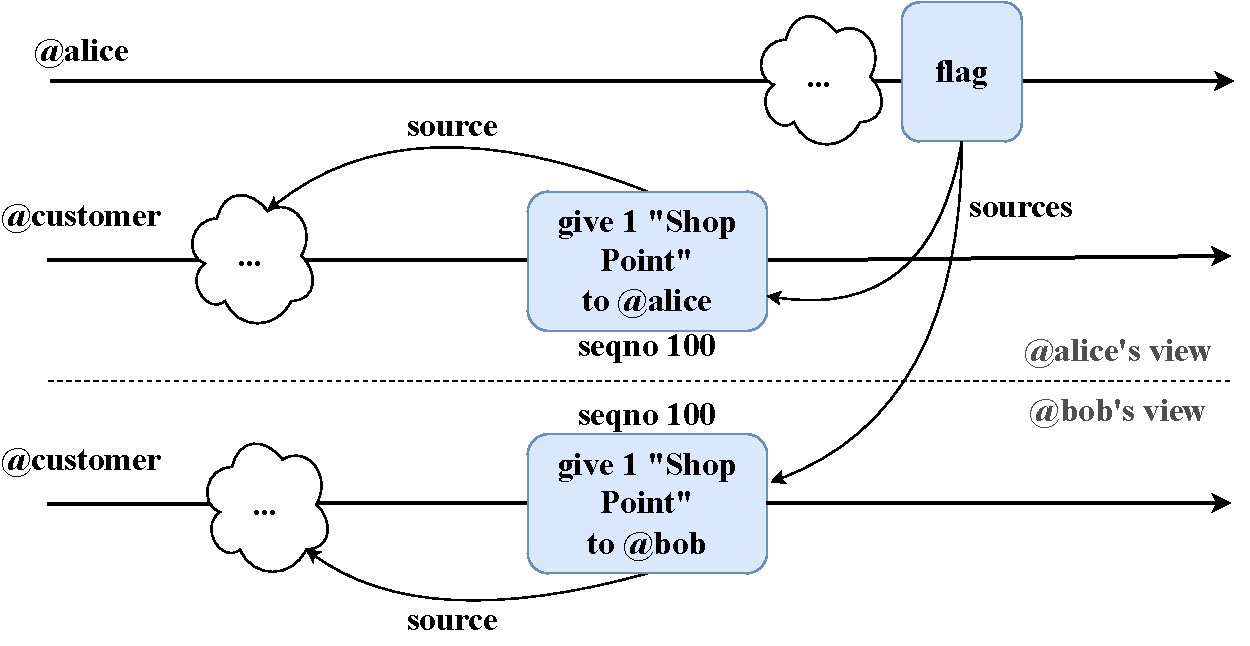
\includegraphics[width=0.48\textwidth]{figures/fork-double-spend-drawio}
\caption{Fork-based Double-Spend}
\label{figure:fork-double-spend}
\end{figure}

The previous examples used append-only logs, but similar issues arise if the system was using replication of sets of authenticated messages instead~\cite{meyer2021setreconciliation}: a malicious participant could selectively present different subsets of messages to different subsets of participants. Nonetheless, because messages are authenticated, eventually two participants in a double-spend will eventually replicate each other's messages and witness that more spendings were done by the malicious actor than the number of tokens available.

\subsection{Comparison to Bitcoin and Ethereum}

In contrast to the previous examples, Bitcoin and Ethereum \textit{prevent} double-spending by making a double-spend attack really costly either in electricity usage or capital lost. The cost of preventing double spending is however quite large: Bitcoin uses in the order of MWh of electricity per transaction, which represents hundred(s) USD worth of electricity depending on local prices, and requires investments in the order of billions of USD of mining equipment (about a hundred USD per address in use);\footnote{As of August 2022, $\approx$ 100 USD/(TH/s) for an ASIC Miner~\cite{bitcoin-asic-mining}, 200M TH/s Total Hashrate of Bitcoin Network~\cite{total-hashrate}, 180M total addresses~\cite{bitcoin-stats} (compared to $\approx$ 1M daily active addresses~\cite{bitcoin-daily-active-addresses}): $\approx$ 110 USD/address (19.8k USD/daily active address).} Ethereum's proof-of-stake uses a minimum of 1.37Wh of electricity per transaction instead~\cite{ethereum-energy-consumption}, but needs a similar capital investment used as collateral stakes to disincentivize cheating.\footnote{As of August 2022, 15B USD Total Capital Stake~\cite{proof-of-stake}, 84.3M total addresses~\cite{ethereum-addresses} (compared to $\approx$ 500k daily active addresses~\cite{ethereum-daily-active-addresses}): $\approx$ 178 USD/address (30k USD/daily active address).} At the moment, the capital investments in mining equipment and stakes are mostly rewarded by the minting of new tokens. However, since the supply of tokens in both cases is artificially limited, eventually the networks will have to pay for their operations only from transaction fees. Assuming miners expect 5-15\% of returns per year on the capital they invest, that translates to fees of at least 5.5-26.7 USD per year per address in use. These fees alone would make a fidelity card program in a sandwich shop unaffordable. From this analysis, we conclude that evolutions of Bitcoin and Ethereum networks in the future will be reserved for larger global transactions, possibly worth hundreds of USD or more.

We postulate that within a local community, \textit{i.e.}, participants that know each other and repeatedly transact over a long period of time, a proof of past double-spending is sufficient to disincentivize cheating\footnote{A cheater may try to create an unknown identity prior to performing a double-spend. However, the transaction from their known identity to the unknown identity will still leave a trace that comes back to them. Moreover, other participants might be suspicious of trading with an identity that has no prior history and refuse to accept the cheater tokens.} because the opportunity cost of loosing the ability to transact with other community members will be worth much more than the gains that can be obtained from the value of most of the transactions performed. Therefore, for small-valued transactions, it is sufficient to simply detect double-spending and propagate proofs that it happened, making the infrastructure required for local economics cheaper. Moreover, requiring eventual detection instead of prevention enables \textit{local-first} operations~\cite{kleppmann2019local-first-software}, without the need for an Internet connection.

\section{Properties of Local Crypto-Tokens}
\label{section:problem}

In this section, we extract from the previous discussions some desired properties of local crypto-tokens, by generalizing those required for the fidelity card program (Section~\ref{section:motivation}):

\textbf{Creator-bound unlimited tokens}: Local crypto-tokens are created by a specific identity, called an \textit{author}, representing a participant or an organization. That identity can create as many tokens of the same type as they require, over multiple operations. This is in contrast to linking the creation of tokens to a mining process, as in Bitcoin, or a smart-contract, as in Ethereum.

\textbf{Trust-based value}:  The value of the tokens depends on the trust that other participants have that the creator will fulfill any promise associated with the tokens, and the willingness of participants to transact with them. This way, the tokens can represent a form of \textit{i-owe-you} (IOU) from the creator to other participants. This is in contrast to the value of tokens deriving from market valuation of a limited supply of a single token, as in Bitcoin, but is similar to many ERC-20 Ethereum tokens~\cite{erc20} that are linked to the services provided by a platform or organization.

\textbf{Unforgeable}: No other identity can create tokens in place of an author, and all transfers between participants use tokens that were explicitly created by an author. This is similar to both Bitcoin and Ethereum tokens, although it is linked to a different creation mechanism.

\textbf{Eventual double-spending detection}: If two honest participants receive tokens from the same source with a total amount larger than what was originally available, the operations involved will be eventually detected by both participants. If some operations can be shown to have happened before the others, the earliest are valid and the latest invalid. Otherwise, all concurrent operations are invalid. This is in contrast to Bitcoin and Ethereum where double-spending can only be done in conjonction with an expensive attack on the network, and for all practical purposes prevented. 

\textbf{Efficient}: We envision local crypto-tokens to run on affordable hardware; consume little energy per transaction, in the order of milli-Wh per transaction; with fast operations, with latency in the order of seconds; and with reasonable memory usage, even in the presence of adversaries. 
In addition, minimal infrastructure shall be required to enable transactions, in the order of a hundred dollars for the devices of participants with minimal need for additional infrastructure. Creating new designs that ensure the previous security properties with low latency, energy, and capital constitutes the main area of research.

We summarize how local crypto-tokens compare to Bitcoin and Ethereum in Table~\ref{tb:properties}.

\begin{table*}[t]
\caption{Summary of properties of \textit{local crypto-tokens} in contrast to Bitcoin and Ethereum ERC20 Tokens.}
\label{tb:properties}
\begin{tabular}{l|r|r|r|}
              & \textbf{Bitcoin} & \textbf{Ethereum ERC20 Tokens} & \textbf{Local Crypto-Tokens} \\
\hline
\textbf{Creation}        & Miners                              & Smart-Contract         & Participants \\
\textbf{Supply}           & Limited                             & Contract-Specific      & Unlimited \\
                                   &                                         & (Limited or Unlimited) & \\
\textbf{Value}             & Market (Artificial Scarcity) & Market Demand for Service(s) & Creator-bound \\
\textbf{Unforgeable}   & Yes                                   & Yes                                                             & Yes \\
\textbf{Ledger(s)}            & Single Global               & Single Global                        & Multiple Local \\
\textbf{Transaction Latency} & tens of minutes      & tens of seconds                                                      & seconds \\
\textbf{Double-Spending} & Prevented                 & Prevented                                                 & Eventually Detected \\
\textbf{Transaction Energy} & MWh  ($10^{6}$)                             & Wh                                                  & mWh ($10^{-3}$) \\
\textbf{Infrastructure Capital} & $\approx$ 110 USD/address
                                    & $\approx$ 178 USD/address   
                                    & <100 USD / participant \\
                                    & (Mining)      &  (Capital Stake)  & (Participant Device)  \\
\textbf{Internet} & Required                            & Required                                  & Optional \\
\end{tabular}
\end{table*}

\section{Applications}
\label{section:applications}

In this section, we present additional applications that could benefit from token implementations that achieve the properties mentioned in Section~\ref{section:problem}.

\subsection{Tracking and Rewarding Open Source Contributions}
\label{section:tracking-oss-contributions}

An open source maintainer creates tokens representing the number of hours volunteers have spent helping improve documentation, report and triage issues, submit patches for code improvements, etc. After validating the contributions, they create the required number of tokens and give them to volunteers. If or once a project receives money from donators, a "buy-back" program can distribute the money by allowing volunteers to exchange their contribution tokens for money at a fixed rate and up to a certain limit, possibly following the ratio of their total contributions compared to other volunteers.

\subsection{Community Crowdfunding}
\label{section:community-crowdfunding}

A project initiator creates tokens that represent the future services that they plan to offer to the community, such as rides on a renovated sailboat.\footnote{This actually happened in the SSB community, albeit without proper token support.} Each token represents a certain amount of value,  \textit{e.g.}, "1 day and night on the sailboat" or "10 Euros" of hosting/sailing services. The initiator sells their tokens to their community in exchange for other currencies or resources to carry the task. Once the sailboat is put in service, community members can exchange their tokens for the promised service. Alternatively, even before the project is actually completed, they can exchange tokens with other community members, for example, if they do not think they will need or want the services anymore.

\subsection{Token-supported Mesh Storage and Retransmission}

Tokens can be used to incentivize participation of nodes in a mesh of wireless nodes. The tokens are used to compensate  costs incurred to store messages in transit and transmitting them to other nodes. Tokens can be emitted by each node independently and therefore represent a promise from a specific node that it will carry traffic in the future. Nodes can "pay" for storage and transmission using tokens created by themselves or by transferring back to other nodes the tokens they themselves created. Nodes individually accept tokens from any other node up to a limit after which traffic is not carried anymore, until the other nodes accept carrying traffic, paid with their own tokens, or they start paying for traffic using other nodes' tokens (obtained also after carrying traffic). In effect, this scheme implements a mutual credit system, including credit limitations.

A second alternative is to have one or multiple external parties, not participating in the mesh, creating tokens with which to pay for traffic. Nodes accept to carry traffic in exchange for those tokens and users of the mesh, source and/or destination for packets, can pay for delivery of traffic by paying the nodes on one or multiple paths between the users.

\section{Related Work}
\label{section:related-work}

In this section, we present work that is related in its objectives and implementation techniques.

\textbf{Secure Scuttlebutt}, in the eventually consistent replication\footnote{Equivalent to asynchronous reliable broadcast.} abstraction it implements using append-only logs~\cite{kermarrec2020gossiping} and the larger decentralized applications ecosystem it spawned~\cite{tarr2019ssb}, can provide both the foundational layer for gossiping token operations as well as an enthusiastic community to experiment with.

\textbf{Producer Credits} as proposed by Paul Grignon~\cite{producercredit} is a major inspiration for the articulation of \textit{local crypto-tokens}, specifically regarding the self-creation of credits by economic actors as promises for their own future production and services. Our formulation however supports additional use cases, such as tracking contributions in open source project (Section~\ref{section:tracking-oss-contributions}) in which a project maintainer instead creates tokens as a form of recognition of quantified contributions to the project. Grignon draws some inspiration from E.C. Riegel. Contrary to E.C. Riegel's and other kinds of mutual credit proposal~\cite{mutualcredit}, Producer Credits can be deployed by individuals without a priori coordination with other economic actors, similar to fidelity programs (Section~\ref{section:motivation}), which makes bootstrapping an economic community easier.

\textbf{Local Currencies} are closely related as well, private fidelity programs being sometimes classified as local currencies. A community create local crypto-tokens to issue currencies that could then be circulated in the community. Local crypto-tokens however does not require \textit{a priori} coordination of a community to be adopted, and can be used for other applications than local currencies.

In contrast to \textbf{Crypto-currencies and Smart-Contracts}, such as Bitcoin~\cite{nakamoto2008bitcoin} which implements a global replicated ledger, and Ethereum~\cite{buterin2014next} which implements a global replicated state machine, local crypto-tokens work with intermittent local connectivity, do not require solving cryptographic challenges (proof-of-work) or providing capital as collateral (proof-of-stake). However, the compromise is that double-spending is \textit{detected} after transactions have been recorded, instead of \textit{prevented}. Mechanisms based on online third-party witnesses shared by all participants, as implemented by \textit{Astro}~\cite{collins2020online}, could add double-spending prevention still without requiring proof-of-work or proof-of-stake, at the cost of relying on cloud infrastructure and Internet connectivity.

Similar to our \textbf{Token-supported Mesh} application proposal, Nuglets~\cite{buttyan2001nuglets} also uses tokens to retribute mesh network nodes for their services. In contrast to Nuglets however, we envision each node to emit tokens for their own services and individually choose whose other nodes' tokens (and associated traffic) they are going to accept and up to which limit. In Nuglets, token transfers are performed in a secure environment to prevent nodes from creating tokens and free-riding on the services offered by other nodes. With \textit{local crypto-tokens}, nodes instead only create tokens for services that they themselves provide. Moreover, nodes cannot forge tokens associated to other nodes or a third-party. There is therefore no need for a secure environment to update token holdings. 

\section{Conclusion and Future Work}
\label{section:conclusion}

In this paper, we formulated the design of new \textit{local crypto-tokens} as a research problem based on unique characteristics of local economics, such as repeated interactions between participants that know and trust each other. We motivated our analysis from a fidelity card problem and other applications. Compared to existing solutions, such as pen and paper fidelity cards, crypto-tokens can provide better security guarantees. Compared to existing blockchain infrastructure, such as Bitcoin and Ethereum, local crypto-currencies could provide faster and cheaper transactions, lower energy usage, and require less infrastructure capital. The need for global transactions between untrusting parties shall however remain, so we expect local crypto-currencies to be useful for intra-community low-value transactions while evolutions of current blockchain projects shall remain useful for inter-communities high-value transactions.

Research shall lead to new local crypto-token designs with low latency, low energy use, and low capital requirements while ensuring the required security properties of unforgeability of tokens and eventual double-spending detection. Ongoing peer-to-peer projects, such as Secure-Scuttlebutt~\cite{tarr2019ssb} or Hypercore~\cite{hypercore}, may serve as interesting foundations but local crypto-tokens could also be implemented on any other infrastructure that provides eventually consistent replication of local messages.

% TODO Add acknowledgement to thank all reviewers and friends for reviewing drafts of the manuscript

\begin{acks}

We would like to thank the SSB community, Akash Dhasade, and the anonymous reviewers for their comments on an earlier draft of this paper.

\end{acks}

\bibliographystyle{ACM-Reference-Format}
\bibliography{main}

\end{document}